Having completed the statistical analysis of the data, a natural question arises: how is it possible to convey the results observed in the analysis to coaches and athletes so that they can obtain an understanding of the data that they have collected? Visualization is an important part of any data analysis as it can offer rapid and meaningful insight into the data due to the inherent human dependency on vision for interpretation. Typically datasets will have multiple dimensions and facets, so in order to gain a broad insight into the data, multiple graphs and images are necessary. Any data visualizations will ideally be portable, system independent and reusable. The options explored for constructing such a system were:
\begin{enumerate}
	\item Building a web application using well-established web development tools such as Ruby on Rails, or Django. This option was not implemented as it would require extensive quantities of boilerplate code.
	\item Creating an executable program that can be run locally. This had a drawback in that the system would somehow need to be distributed, which went beyond the scope of this project.
	\item Building a web application using a customized web framework such as Spyre or Shiny. Shiny is a package within R, an open source statistical language and development framework, that facilitates the development of reactive data visualizations through a web browser. This was the most attractive choice of the three. Since the data analysis was performed using R, Shiny was chosen to develop the application.
\end{enumerate}

\section{Shiny}
Shiny is an open source R package that provides a high level web development framework. Shiny was developed with the aim of converting analyses into interactive web applications with minimal knowledge of HTML, CSS, Javascript and other common web-development languages. The focus is on presenting graphics to the end user which can enlighten them about their data. The advantages of using Shiny are:
\begin{itemize}
	\item It's interactive which means it can offer a dynamic user experience. 
	\item Shiny applications are written in R and can utilize all of the libraries that are already available in the R language.
	\item The development of a shiny App is centered around displaying graphics generated with R to the user. If you can program with R, you can program with Shiny.
\end{itemize}
Since R was used to perform the statistical analysis, it was a natural extension to develop the visualizations using the Shiny package. Every Shiny application consists of a minimum of a server function and a user interface function which follows the ``separation of concerns" design principle. The server is concerned with data manipulation and mapping user inputs to various types of output, whereas the user interface is concerned with data presentation. I followed the convention in Shiny of creating a project folder and then writing R files named server.r, ui.r and a www folder which contains css and image files used by the browser in the App, found at \cite{ShinyServer}\cite{ShinyUI}.

\section{Functionality}
In the application that I developed, I set out a certain amount of functionality that would be necessary to make the App straightforward for the user to operate. The following subsections offer an exposition of how this was achieved.

\subsection{Dropbox File Upload}
It was necessary for  the App to allow the user to upload their own csv file in order to display their data. This was easily be achieved through using a local file uploader, which Shiny provides using the fileInput widget. However, only facilitating local file uploads imposed limitations: it is undesirable for a sports team's data to be located on a number of different machines rather than on a central repository, the most obvious consequence being that if one of the machines is damaged, data could be lost permanently. For these reasons, tools like Dropbox are often used to store and access athlete data. I decided to add the option to upload data from the users' Dropbox account to the App. This required using the package rdrop2 to facilitate the user logging into their dropbox and permitting the App to upload data from their dropbox to the App. This was achieved using the following code segment:

\begin{lstlisting}[language=R, basicstyle=\tiny]
dropboxDown=reactive({
  if(input$dropboxDownload){
  #only run this authorization once (not sure how to do this without the use of global variable)
    if(!alreadyVisited){
      #consider adding new_user=TRUE
      dropbox_credentials=drop_auth(cache=FALSE)
      updateCheckboxInput(session, "dropboxDownload",label='Choose a file:')
      #update file choices
	  updateSelectizeInput(session,'dropboxFileSelection',choices=basename(
	  drop_search('.csv')[order(drop_search('.csv')$modified),]$path))
	  #set global alreadyVisited variable to TRUE as this behaviour should only occur once
	  alreadyVisited<<-TRUE
	}
	#update the input file to the file selected by the user
	inFile1=input$dropboxFileSelection
	#check file exists
	if (is.null(inFile1)){
	  print('No file provided')
	  return(NULL)
	}
	else{
	  #can deal with RData and csv formatted files
	  if(length(grep('.csv',inFile1))!=0){
	    #read csv by finding the path in dropbox, ensure ProcessedData is global
	    ProcessedData<<-drop_read_csv(drop_search('.csv')[match(inFile1,basename(
	    drop_search('.csv')$path)),]$path,stringsAsFactors=FALSE)
	    #be careful as write.csv adds an x column if column.names=FALSE
	    ProcessedData$Date=as.Date(ProcessedData$Date)
	  }
	  else if(length(grep('.RData',inFile1))!=0){
	    load(inFile1$datapath)
	    ProcessedData<<-ProcessedData
	  }
    }
    if(exists('ProcessedData')){
	  #If the data exists, preprocess it
      Preprocess()
      #now allow the user to download a report
      shinyjs::enable("report")
      shinyjs::enable("refreshReport")
      #call data preprocessing function, look into passing Preprocess to this function
    }
  }
})
\end{lstlisting}
This led the user through the sequence of events displayed in figures 3.1-3.4: 
\begin{figure}[h]
	\centering
	\begin{minipage}{.48\textwidth}
		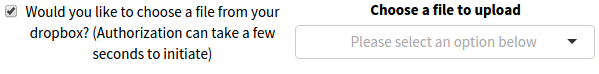
\includegraphics[width=1\linewidth, height=1cm,left]{Images/RDropCheckbox.png}
		\caption{1). Click checkbox}
	\end{minipage} %
	\hfill
	\begin{minipage}{.4\textwidth}
		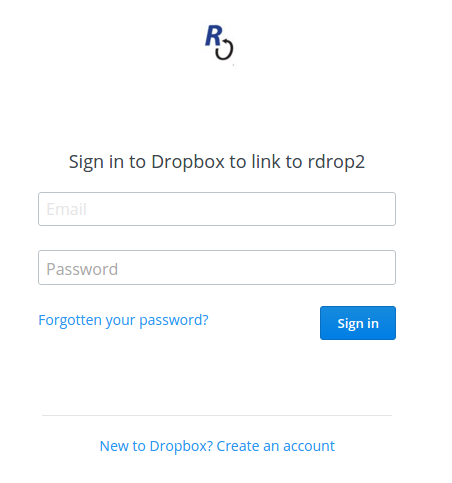
\includegraphics[width=0.9\linewidth, height=3cm,right]{Images/RDropLogin.png}
		\caption{2). Sign in to Dropbox}
	\end{minipage} %
	\newline
	\centering
	\begin{minipage}{.45\textwidth}
		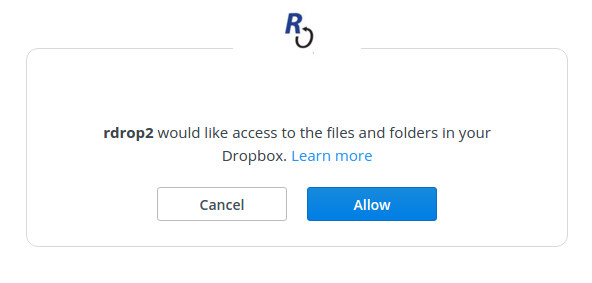
\includegraphics[width=1\linewidth, height=3cm,left]{Images/RDropAuth.png}
		\caption{3). Authorize file access}
	\end{minipage} %
	\hfill
	\begin{minipage}{.45\textwidth}
		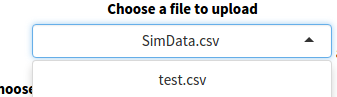
\includegraphics[width=1\linewidth, height=2cm,right]{Images/rdropDropDown.png}
		\caption{4). Upload Dropbox file}
	\end{minipage}
\end{figure}

\break\hfill

The rDrop2 package stores tokens containing the users password and user name so that the user does not have to log in every time the App is used, however this caused security issues regarding the safe storage of these details. There are options in the function drop\_auth which prevented the caching of login details by the application and also the option of specifying whether a new user is logging in (and whether previously cached details should be overwritten). In practice however, it seemed that the application created a file named .httr-oauth containing the cached user login information regardless of these options. This would be a major issue if the code was used in production but since the application was proof of concept, it was not resolved.

\subsection{CSV Upload Format}
The user must upload the data in a certain file format for this application to be able to process the file. From the outset I intended to write an application that would impose a minimum amount of restrictions on the user with the intent of having a scalable and extendable program. The modularity of the code has the consequence of decoupling the displays from the variables that are being displayed. In the application functions took as input the name of any numeric column in the data and outputted graphs. This meant that the only variables that must necessarily be present in the data are Date and Name (of athlete). The consequence of this is that the application can be modified in a matter of minutes to display the same graphs and summaries for a csv file containing any type of numeric Athlete data. 

\subsection{Application Tabs}
The rest of the functionality of the application was modularized into tabs which could be navigated in order to display a specific plot or summary.
\newpage
\subsubsection{Longitudinal Plot}
\begin{wrapfigure}{r}{9cm}
	\vspace{-2em}
	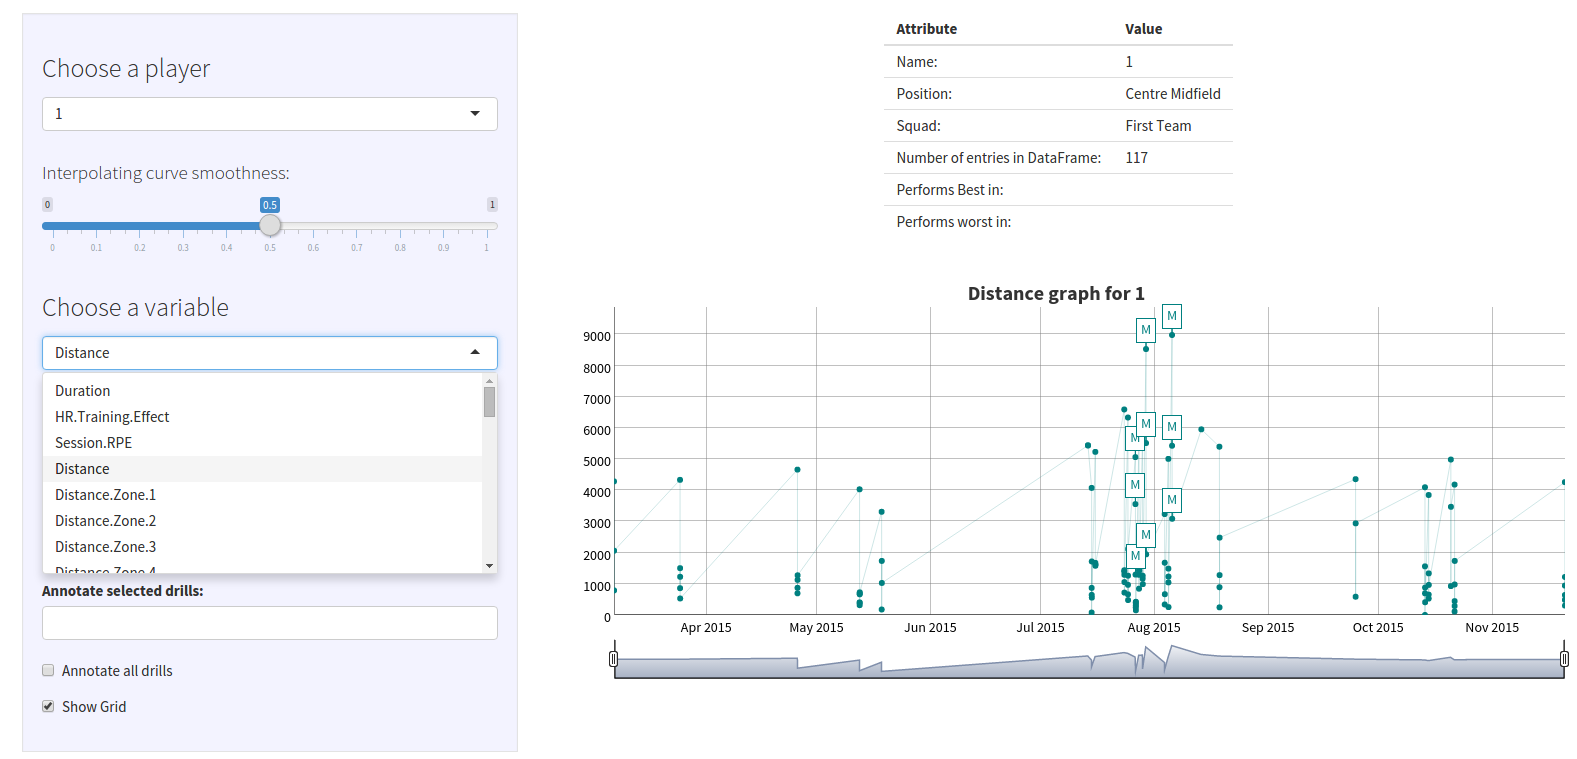
\includegraphics[height=5cm, width=10cm]{Images/PlotTab.png}
	\caption{Longitudinal Plot Tab}
\end{wrapfigure}
The tab that the application navigates to by default displays a longitudinal plot. This plot gives the user graphical information about how some aspect of the athletes' training has changed over time. The user can subset the graph to a certain date range and has the option to compare another athlete on the same graph. The option is also given to annotate drills so that if there is an unusual looking data point, the application user can immediately figure out which training session the unusual data originated from. The R dygraph package was the main tool used to achieve this. 

\subsubsection{Training Calendar}
\begin{wrapfigure}{r}{9cm}
	\vspace{-2em}
	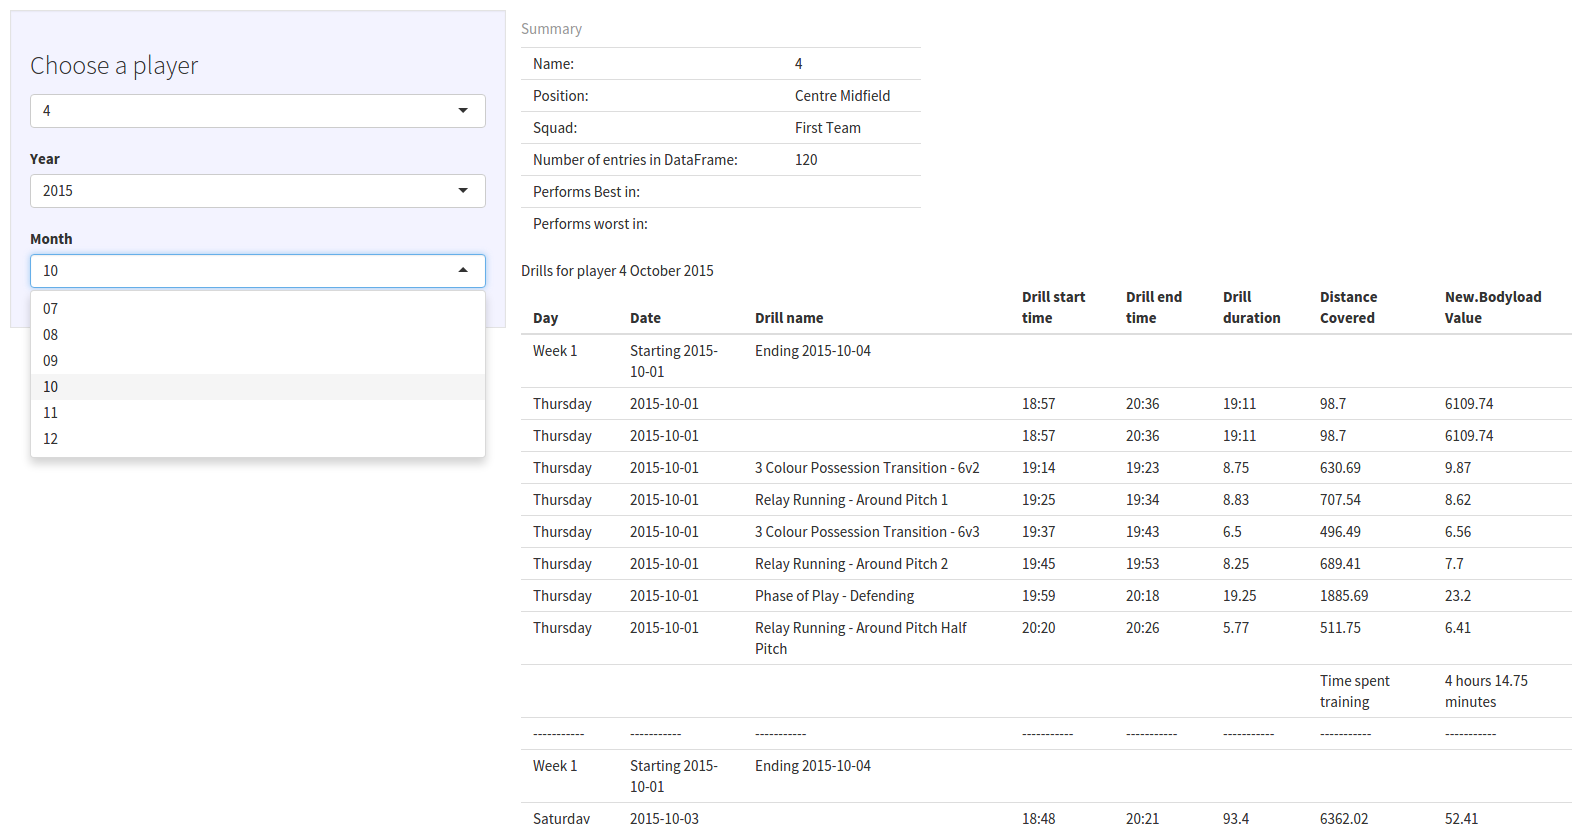
\includegraphics[height=5cm, width=10cm]{Images/TrainingCalendarTab.png}
	\caption{Training Calendar tab}
\end{wrapfigure}
The training calendar tab provides the user with a readable account of an individual athlete's training schedule over a month in the data provided. The calendar displays which drills the athlete performed, the drill start and end times, the total duration of the drill, the distance that the player covered in the drill as well as the New.Bodyload value generated for that drill. The calendar is broken into weeks of the month so that athletes and coaches have a week-by-week account of the drills that were performed. The code was written so more details about the training session can be conveniently added.


\subsubsection{Bar Plot}
\begin{wrapfigure}{r}{9cm}
	\vspace{-2em}
	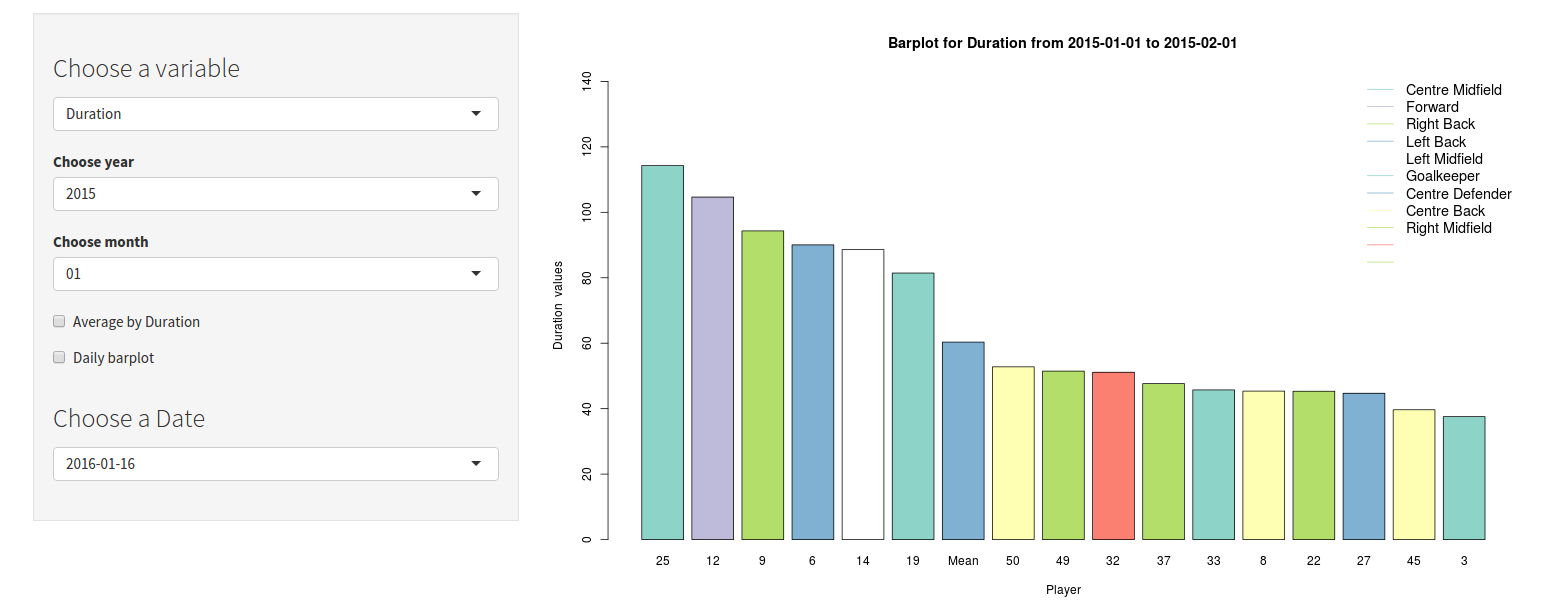
\includegraphics[height=5cm, width=10cm]{Images/BarplotTab.png}
	\caption{Bar Plot tab}
\end{wrapfigure}
The bar plot tab was designed to give a graphical representation of how players in the team performed relative to each other over a date range for a certain variable. This is useful as sometimes absolute figures can lose meaning whereas comparing each player in the team to other players in the team quickly informs coaches who is under performing in certain aspects. The bar plot is coloured by position so that it is easy to compare players competing for the same position. There is an option to average the displayed variable by duration because, as discussed in 2.2.2, accumulative variables are not measured according to the same scale when mean values are taken. Therefore this plot can be somewhat misleading and should be used with caution. There is also an option to view the data with greater granularity by selecting to display the bar plot over an individual date.

\subsubsection{Rankings}
\begin{wrapfigure}{r}{9cm}
	\vspace{-2em}
	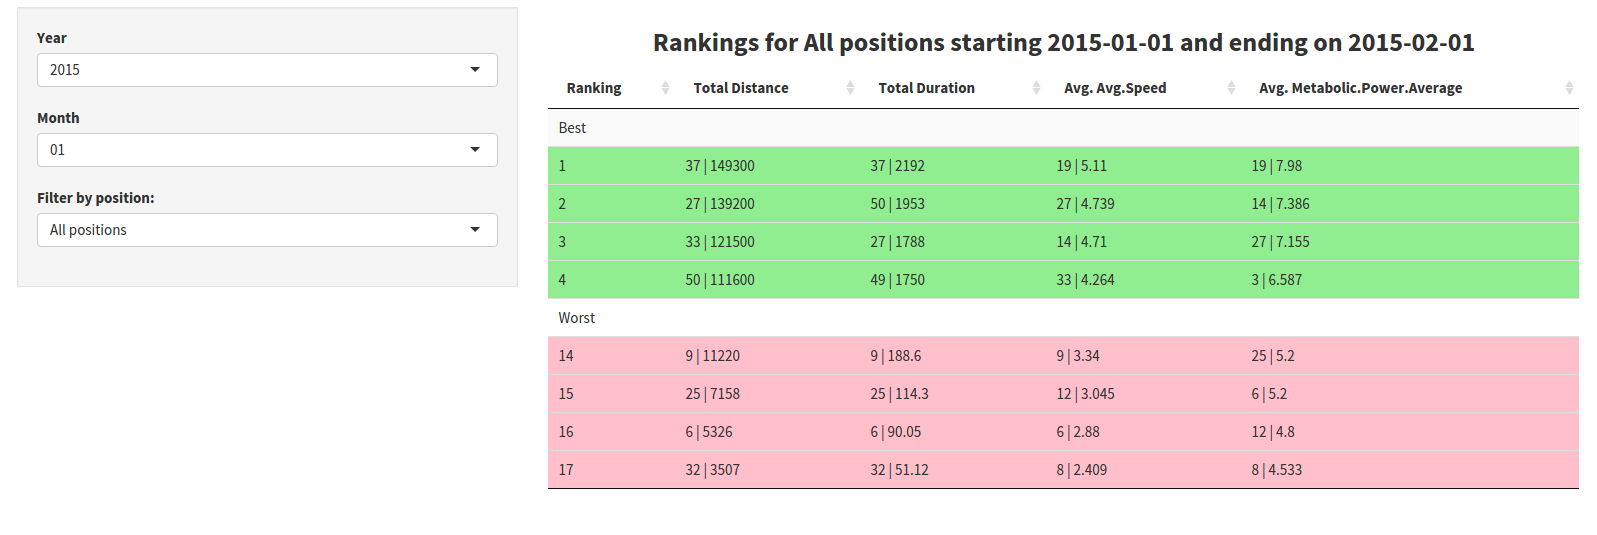
\includegraphics[height=4.5cm, width=10cm]{Images/RankingsTab.png}
	\caption{Rankings tab}
\end{wrapfigure}
The rankings tab was designed to display information about some key variables in the data in a compact and succinct manner. The figure was generated using the DT package in R. The user is given the choice to subset the time period to a month and the players who achieved the best and worst values in each key variable are highlighted. The name of the player is displayed beside the value that the player achieved for the variable over the time period. Again, care must be taken when using accumulative variables as the means of theses variables cannot accurately be compared.


\subsubsection{Report Downloader}
\begin{wrapfigure}{r}{9cm}
	\vspace{-2em}
	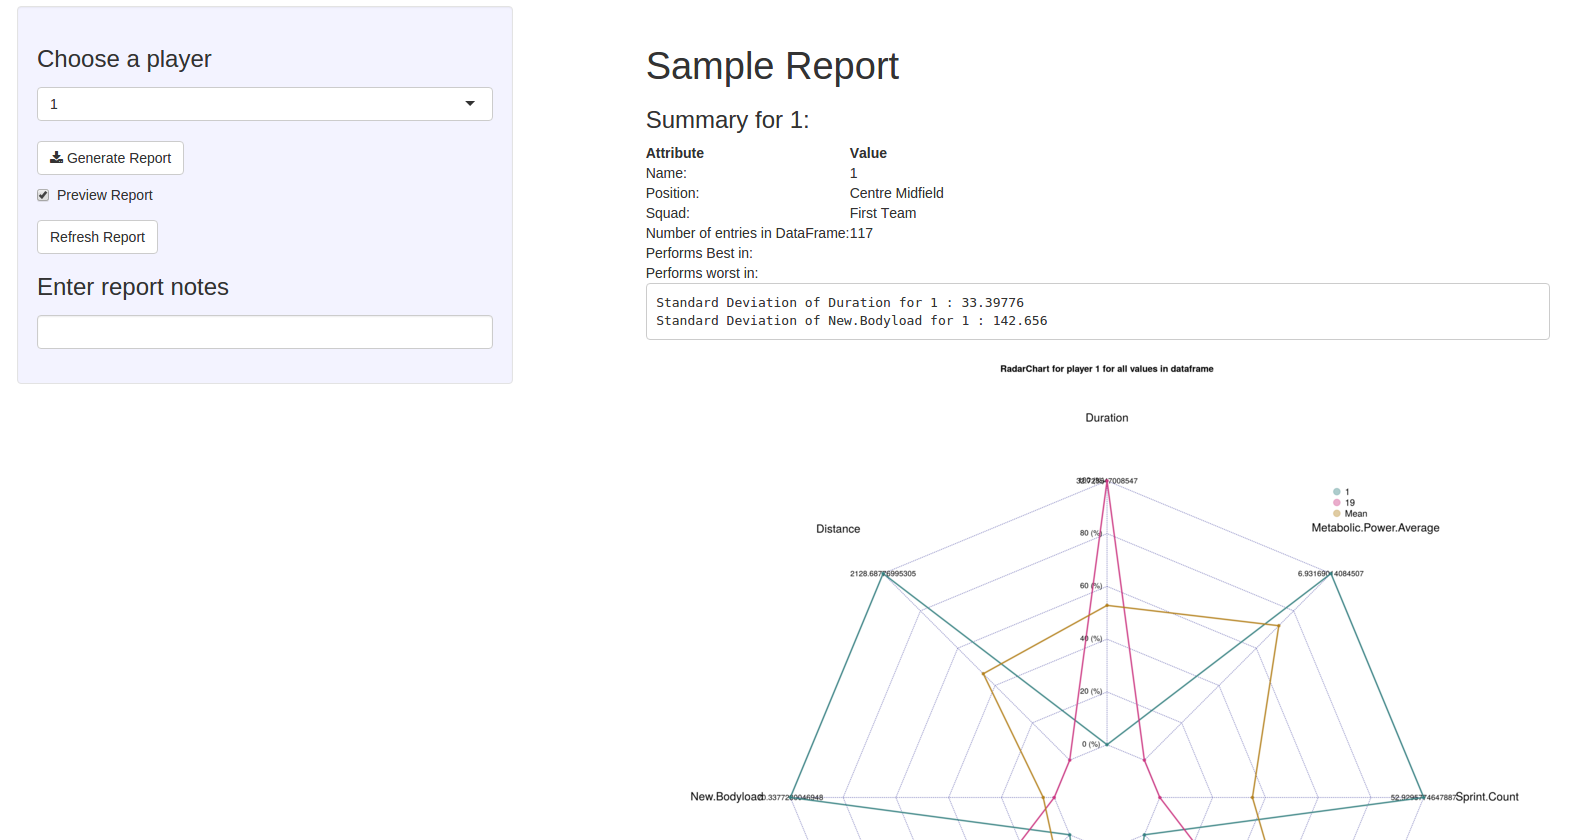
\includegraphics[height=5cm, width=10cm]{Images/DownloadReportTab.png}
	\caption{Report Download tab}
\end{wrapfigure}
The report Downloader tab facilitates the user entering some notes about a player and then downloading a customized report for that player. There is an option to view a rough preview of the report before downloading it, as shown in Figure 3.9. The report itself was generated using RMarkdown and introduces significant overhead to the App. A caching system for the reports or a separate report generating mechanism that runs in parallel to the application would be desirable for this tab, however to achieve this would take a considerable amount of code. There are also security issues related to downloading the report and the mechanism for storing the reports is currently flawed, meaning this is the only part of the application that would not run if deployed to a server.

\section{Dependencies}
Shiny's key strength is it's ability to display reactive output. This is facilitated using a series of outputs generated by the server function, which will automatically update when any of the inputs that the output relies on changes. This is referred to as dependency in a Shiny application. Dependencies are automatically created by the framework in order to track when an input variable changes so that the corresponding output remains up to date. The only requirement is that each input and output has a unique identifier in the App name space. Dependencies reflect the fundamental relationship between outputs and inputs. For example, in my application the player summary tables changed whenever the selected player changed, hence a dependency was set up on selected player. However, the programmer must be careful to only re-run code when necessary, otherwise a large overhead would be introduced making the program sluggish and frustrating to use. Shiny handles this by providing reactive functions, which come in three main flavours: reactive, render and observe, all of which were used in the application. 
\subsubsection{Reactive Expressions}
\begin{wrapfigure}{r}{4cm}
	\vspace{-2.5em}
	\caption{Example reactive expression \cite{shinyCheatSheet}\label{wrap-fig:1}}
	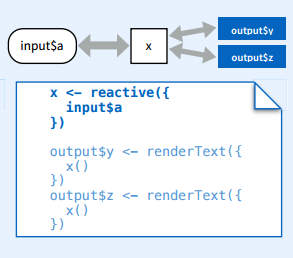
\includegraphics[height=3cm, width=4.5cm]{Images/ReactiveExpressionExample.png}
\end{wrapfigure}

The purpose of reactive expressions is to create objects that will be used in multiple outputs. Reactive expressions cache their evaluations the first time you run them. In subsequent calls, the reactive expression checks if the saved value needs to be updated (i.e., whether the inputs it depends on have changed). If the value does need to be updated, the reactive object will recalculate it and then cache the new result. If the value is already updated, the reactive expression will return the cached value without running the computations involved in the function \cite{shinyCheatSheet}. In my application, the Preprocess reactive expression took in data provided by the user and cleaned it so that it was in a suitable format for use throughout the rest of the server. Since this calculation took a few seconds to run in the application, using the cached value greatly boosted the App's responsiveness.
\begin{lstlisting}[language=R, basicstyle=\small]
Preprocess=reactive({
  #do all preprocessing, validation and error checking here and then
  #return processed data frame
  .....
  .....
  ProcessedData
})

\end{lstlisting}

\subsubsection{Observe Expressions}
\begin{wrapfigure}{r}{4cm}
	\vspace{-2.5em}
	\caption{Example observe expression \cite{shinyCheatSheet}}\label{wrap-fig:2}
	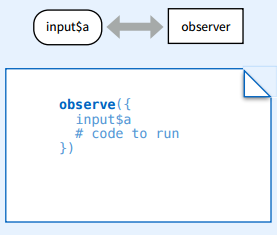
\includegraphics[height=3cm, width=4.5cm]{Images/ObserveExample.png}
\end{wrapfigure} 

Observe expressions create code that executes when an input changes, but do not directly create output objects. Observers are most often used for their side effects \cite{shinyCheatSheet}. For example, in my application I wanted the months drop down to only contain months that athletes trained in for the selected year. An observe expression was used to create a dependency on the barplotyear input. When the barplotyear input changed, the observer ran and updated the barplotMonth input, without returning anything.
\begin{lstlisting}[language=R, basicstyle=\small]
upDateBarplotMonths=observe({
  #Create dependency on barplotyear - when this changes, dates need to
  #update
  input$barplotYear
  validate(need(exists('ProcessedData'),""))
  updateSelectInput(session, "barplotMonth", 
  choices = sort(unique(format(as.Date(ProcessedData[format(as.Date(
  ProcessedData$Date,format="%Y/%m/%d"),'%Y')==input$barplotYear,'Date'],
   format="%Y/%m/%d"),"%m")))
  )
})
\end{lstlisting}
\newpage
\subsubsection{Render Expressions}
\begin{wrapfigure}{r}{4cm}
	\vspace{-2em}
	\caption{Example observe expression \cite{shinyCheatSheet}}\label{wrap-fig:2}
	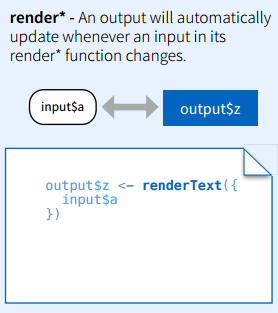
\includegraphics[height=3cm, width=4.5cm]{Images/RenderExpression.png}
\end{wrapfigure} 

Render functions are used in shiny Apps to pass plots, charts, text and other output created in the server to the UI to be displayed. An output will automatically update whenever an input in its render function changes. Render expressions typically hold the code that the server needs to rebuild a UI component after a widget changes \cite{shinyCheatSheet}. Shiny uses the convention of naming render expressions as render[Output Type], where the output types range from tables to plots. Render expressions must return a specific type of object to be displayed or else errors are incurred. In my application, the render expressions tended to be lengthy since most of the plots are quite detailed, however a simple example exists in the form of the player summary table.
\begin{lstlisting}[language=R, basicstyle=\small]
output$PlayerSummaryPlot=renderTable({
  input$getname
  playerSummary(input$getname)
})
\end{lstlisting}

\subsubsection{Dependency Graph}
\begin{wrapfigure}{r}{5cm}
	\vspace{-2em}
	\caption{Render \& Observe Nodes (Endpoint)\cite{shinyCheatSheet}}
	
\includegraphics[height=0.8cm, width=1.5cm]{Images/ReactOutput.png}
	\caption{Reactive Nodes (Intermediary)\cite{shinyCheatSheet}}
	
\includegraphics[height=0.8cm, width=1.5cm]{Images/MidPoint.png}
	\caption{Input Nodes (Start Point)\cite{shinyCheatSheet}}
	
\includegraphics[height=0.8cm, width=1.5cm]{Images/InputNode.png}
\end{wrapfigure}  
Shiny has many debugging tools and tricks that can help the application designer to ensure that their App is running as expected. One such tool is the reactive log visualization. This is essentially a dependency chart that shows how the outputs in an application depend on the inputs. There are three types of nodes in this chart displayed in figures 3.3-3.5. Figure 3.16 displays a dependency graph created before the App was completed. Notice that some nodes have many connections which denotes indicates their complexity in the application. Nodes exist that have no connections which shows that they are redundant in the application (which can be useful for debugging).
\begin{figure}[h]
	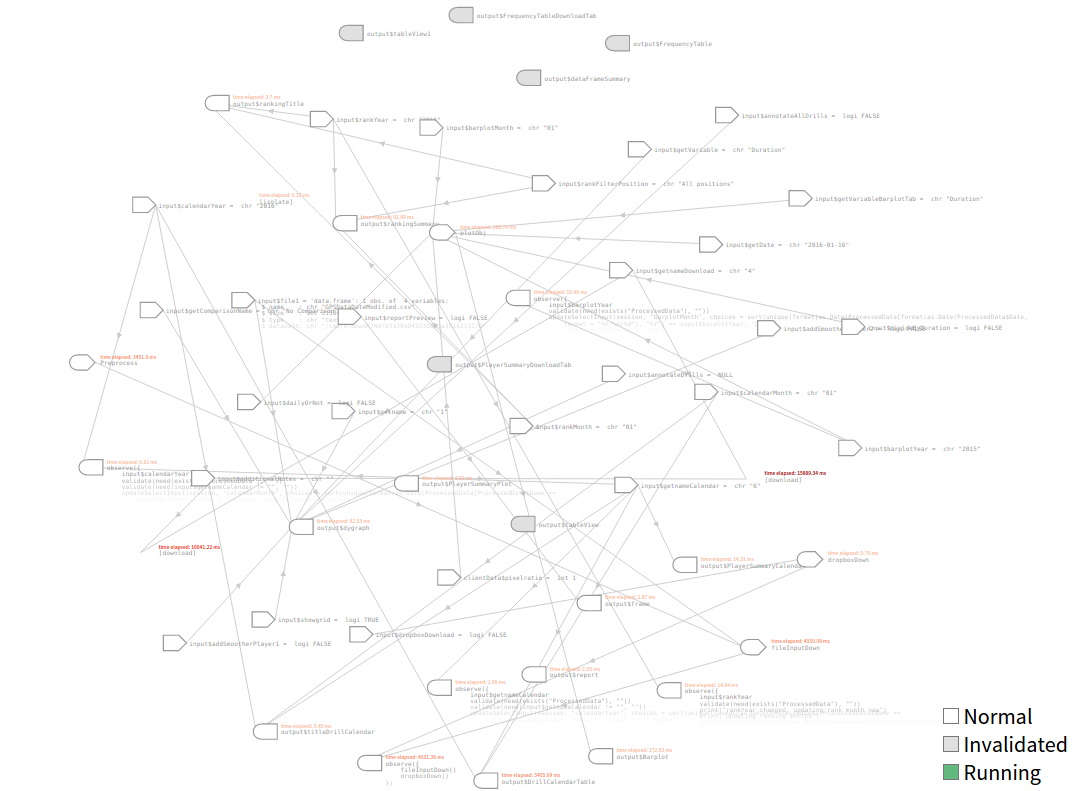
\includegraphics[width=18cm, height=10cm]{Images/ReactLog.png}
	\caption{Reactive Log Graph}
\end{figure}

\section{Program Work-flow}
Shiny applications execute according to the following sequence: 
\begin{enumerate}
	\item The UI file runs everything above the UI function once.
	\item The UI file runs the code inside the UI function once.
	\item The Server file runs the code above the Server function once.
	\item The Server file runs any code outside render, reactive or observe functions once.
	\item The Server file runs code inside reactive expressions multiple times according to the dependency list that Shiny has built up. Whenever an input in a reactive expression changes, the expression will re-run.
\end{enumerate}
The program was designed to comply with this work-flow. Auxiliary functions and other expressions that only need to be run once were defined outside of the server function in order to improve the responsiveness of the App. Reactive expressions contained the minimum amount of code that was required to update the application when a dependency changed in value.

\section{Testing}
As the App grew in complexity, it grew frustrating to alter some section of code and then manually run the App and check each tab to ensure that the App still operated as intended. I wrote a short set of unit tests in the python language using the selenium package in order to automate this process. This meant that every time I made a significant change to the App, I could run the tests while working on some other part of the application without having to manually ensure everything was present. I wrote the tests in python because the application needed to be running in order to use the selenium web driver to navigate it and because python is more suited to testing web applications than R. Code can be found for the tests on Github at \cite{AppTestFiles}.








